\section{Dynamic Hash Table}\label{sec:dyn}
In this section, we propose the resizing strategy against dynamic hash table updates on GPUs. We first present the hash table design in Section~\ref{sec:dyn:has}.
Subsequently, the resizing strategy is introduced in Section~\ref{sec:dyn:resize}.
In section~\ref{sec:dyn:distribute}, we discuss how to distribute the KV pairs for better load balancing with theoretical guarantees. 
Finally, we present how to efficiently rehash and relocate the data after the tables have been resized in Section~\ref{sec:dyn:rehash}. 

\subsection{Hash Table Structure}\label{sec:dyn:has}
Following cuckoo hashing \cite{pagh2004cuckoo}, we build $d$ hash tables with $d$ unique hash functions: $h^1,h^2,\ldots,h^d$. 
In this work, we use a set of simple universal hash function such as $h^i(k) = (a_i\cdot k + b_i \mod p) \mod |h^i|$.
$a_i,b_i$ are random integers, $p$ is a large prime.
Note that the proposed approaches in this paper also apply to other hash functions as well. 
There are three major advantages for adopting cuckoo hashing on GPUs. 
First, it avoids chaining by inserting the elements into alternative locations if collision happens. As discussed in Section~\ref{sec:rel}, 
chaining presents several issues which are not friendly to the GPU architecture.  
Second, to lookup a KV pair, one only needs to search $d$ locations specified by $d$ unique hash functions. 
Thus, the data could be stored contiguously in the same location and enable the preferred coalesced memory access. 
Third, cuckoo hashing can maintain high filled factor, which is ideal for memory saving in the dynamic scenario. 
For $d=3$, cuckoo hashing achieves over $90\%$ filled factor and still processes \formal{insert} operations efficiently \cite{fotakis2005space}.

\begin{figure}[t]
	\centering
	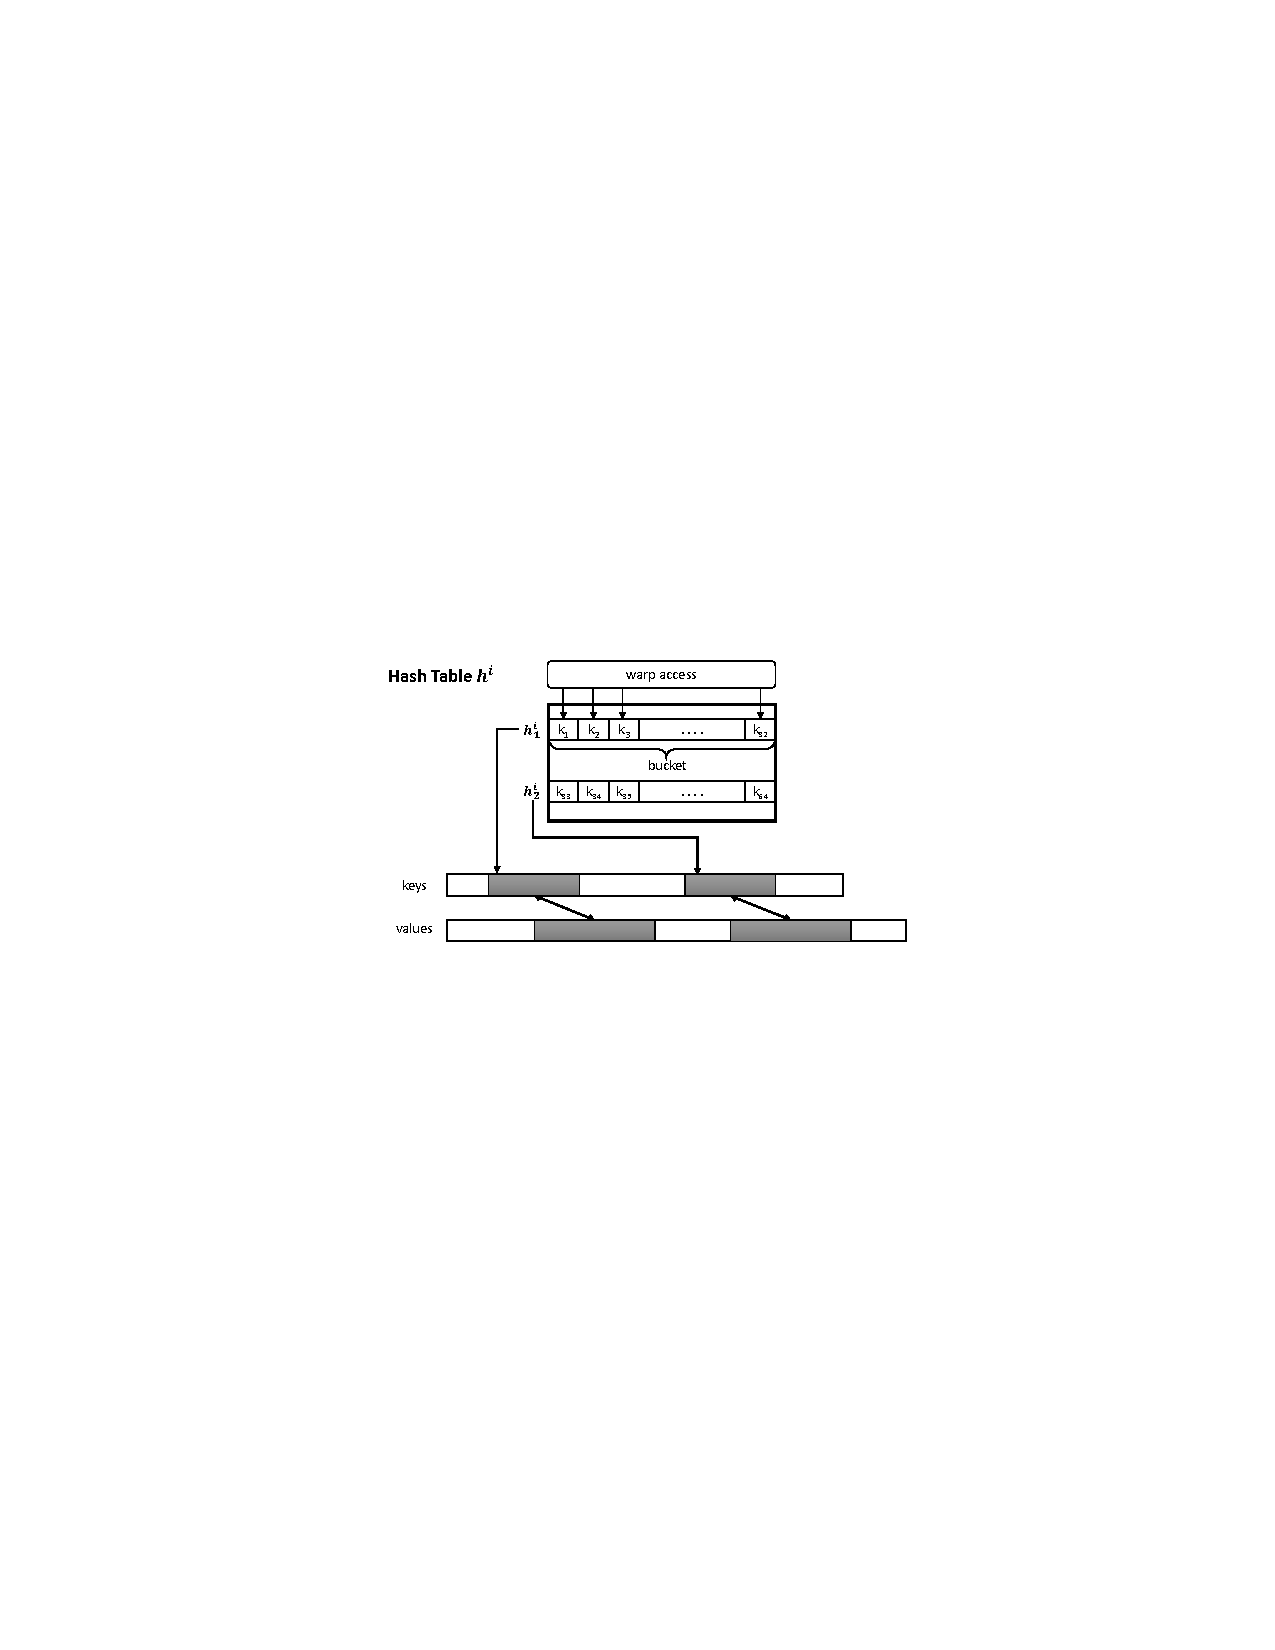
\includegraphics[width=0.45\textwidth]{fig/Hashtable.pdf}
	\caption{The hash table structure}
	\label{fig:hashtable}
\end{figure}

Figure~\ref{fig:hashtable} depicts the design of a single hash table $h^i$ on GPUs. 
Assuming the keys are 4-byte integers. A bucket of 32 keys, which are all hashed to the same value $h^i_j$, are stored consecutively in the memory. 
The design of buckets maximizes the utilization of memory bandwidth in GPUs. 
Consider the L1 cache line size is 128 bytes, only a single access is required when one warp is assigned to access a bucket. 
The values associated with the keys in the same bucket are also stored consecutively but in a separate array.   
In other words, we use two arrays to store the keys and the values respectively.
The values could take much larger memory space than the keys. 
Thus, storing keys and values separately avoid the overhead of memory access when accessing the values are not necessary, 
e.g., finding a nonexistent KV pair or deleting a KV pair. 

For keys having size larger than 4 bytes, a simple strategy is to store less KV pairs in a bucket. Suppose the keys are 8-bytes, a bucket can then accommodate 16 KV pairs. 
Furthermore, we lock the entire bucket exclusively for a warp to perform insertion/deletion using intra warp synchronization primitives. Thus, we do not limit ourselves to supporting KV pairs with only 64 bits. 
In the worst case, a key taking 128 bytes occupy one bucket alone, which is unnecessarily large in practice.

\subsection{Structure Resizing}\label{sec:dyn:resize}
To efficiently utilize GPU device memory, we resize the hash tables when the filled factor falls out of the desired range, e.g., $[\alpha,\beta]$.
One possible strategy is to double or half all hash tables and to then rehash all KV pairs. However, this simple strategy renders poor memory utilization and 
excessive overheads for rehashing. First, doubling the size of the hash tables results in filled factor immediately cut to half, while downsizing the hash tables to half the size followed by rehashing could only be efficient when the filled factor is significantly low (e.g., $40\%$), both of which scenarios are not resource friendly. Second, rehashing all KV pairs is expensive and it hurts the performance stability for most of the streaming applications since the entire hash table is subject to locking. 

We propose an alternative strategy, illustrated in Figure~\ref{fig:resize}. 
Given $d$ hash tables depicted in Figure~\ref{fig:resize},
we always double the smallest subtable or chop the largest subtable into half for upsizing or downsizing respectively, when filled factor falls out of $[\alpha,\beta]$. 
In other words, no subtable will be more than double the size as others. The strategy implies that we do not need to lock all hash tables and only to resize one, thus achieving better performance stability compared with the aforementioned simple strategy. 

\vspace{1mm}
\noindent\textbf{Filled factor analysis:}
Assuming there are $d'$ hash tables with size $2n$, $d-d'$ tables with size $n$ and the current filled factor $\theta$, 
one upsizing process when $\theta > \beta$ lowers the filled factor to $\frac{\theta\cdot(d+d')}{d+d'+1} \geq \frac{\beta \cdot d}{d+1}$.  
Since the filled factor is always lower bounded by $\alpha$, we can deduce that $\alpha < \frac{d}{d+1}$.
Apparently, a higher lower bound can be achieved by adding more hash tables, while it leads to less efficient \formal{find} and \formal{delete}. 
We allow the user to configure the number of hash tables to trade off memory and query processing efficiency. 

\begin{figure}[t]
	\centering
	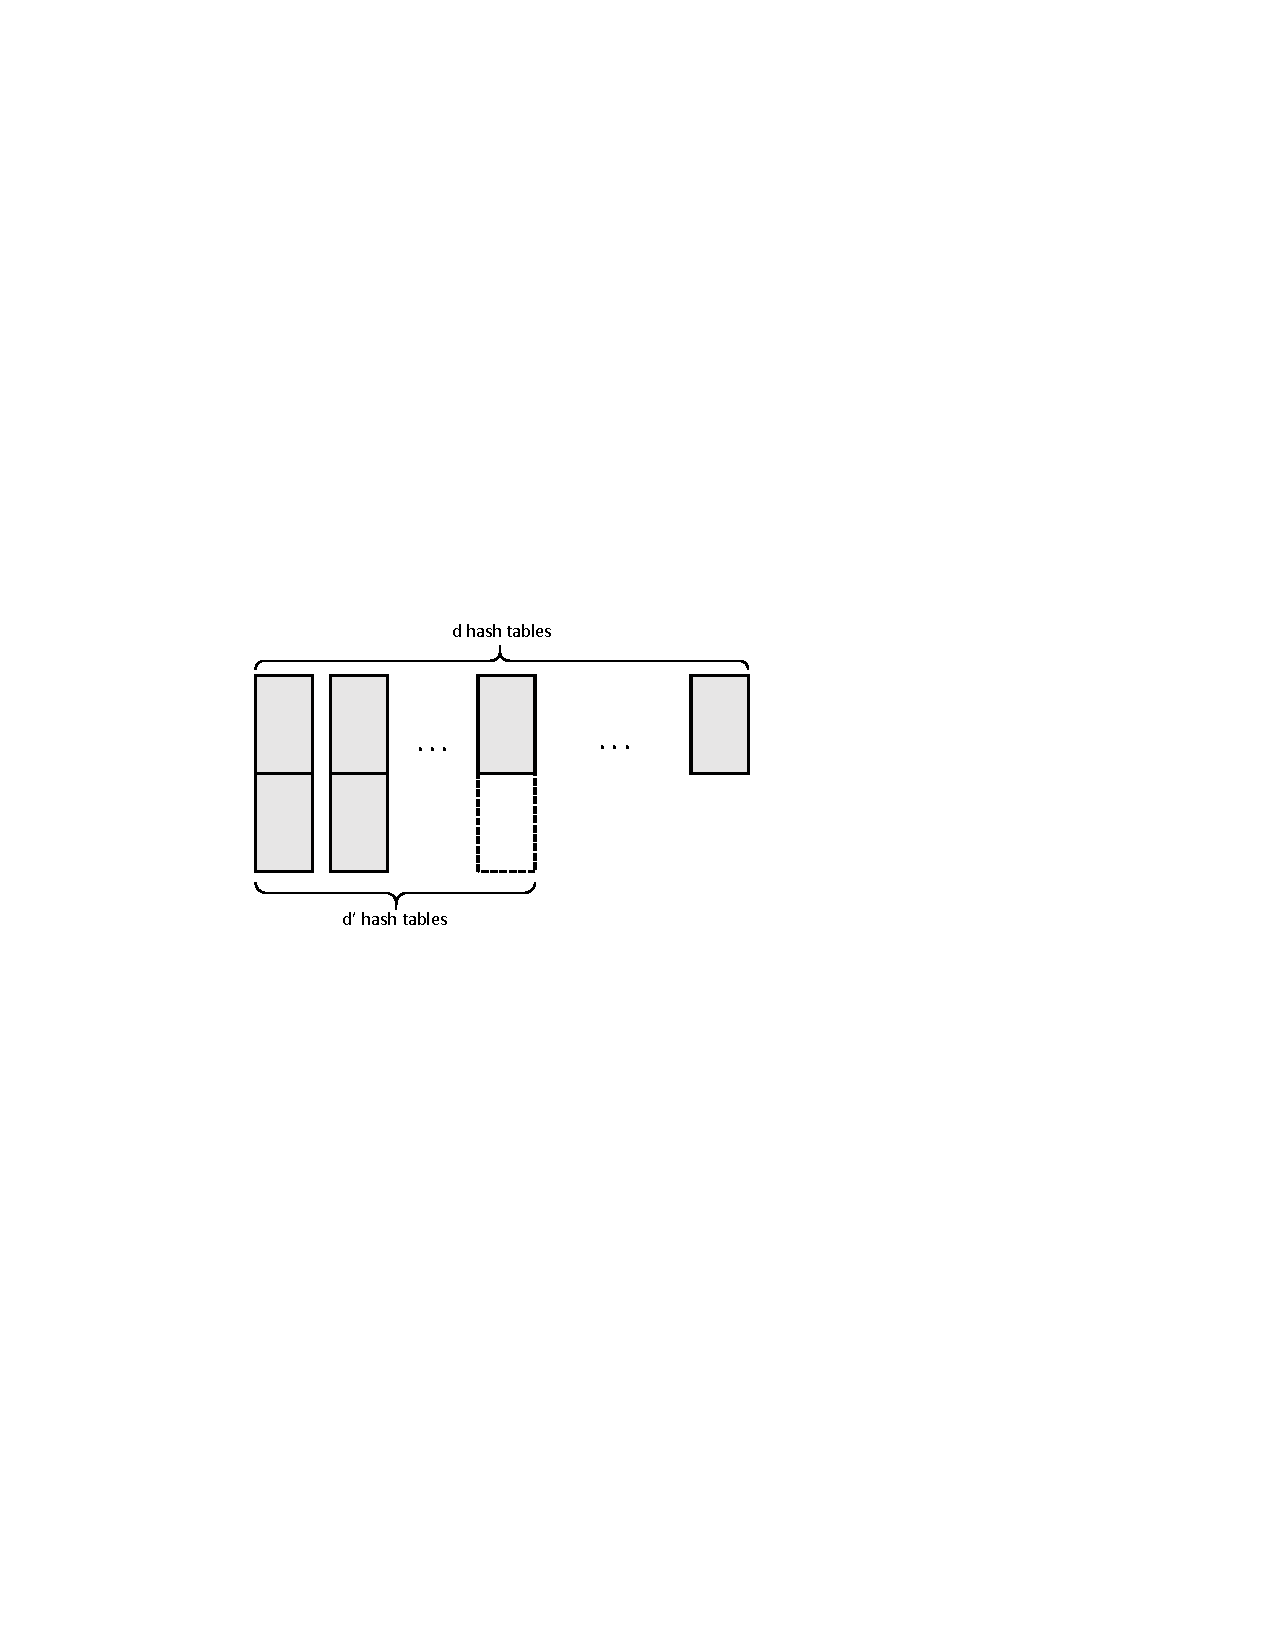
\includegraphics[width=0.35\textwidth]{fig/MultiTable.pdf}
	\caption{Resizing strategy}
	\label{fig:resize}
\end{figure}
\subsection{KV distribution}\label{sec:dyn:distribute}
Given a set of KV pairs to insert in parallel, it is critical to distribute the KV pairs among the hash tables in a way such that the hash collisions are minimized for reducing the corresponding thread conflicts. We have the following theorem to guide us for distributing the KV pairs. 

\begin{theorem}\label{them:balance}
	The amortized conflicts for inserting $m$ unique KV pairs to $d$ hash tables is minimized when $\binom{m_1}{2}/n_1 = \ldots = \binom{m_d}{2}/n_d$. 
	$m_i$ and $n_i$ denote the elements inserted to table $i$ and the size of table $i$ respectively.  
\end{theorem}
\begin{proof}
	It is noted that the amortized insertion complexity of cuckoo hash is $O(1)$. Thus, similar to balls and bins analysis, the expected number of conflicts occurred for inserting $m_i$ elements in table $i$ is estimated as $\binom{m_i}{2}/n_i$. Minimizing the amortized conflicts among all hash tables can be modeled as the following optimization problem:
	\begin{equation}\label{eq:conflict-min}
	\begin{array}{ll@{}ll}
	\min_{m_1,\ldots,m_d \geq 0} & \sum_{i=1,\ldots,d} \binom{m_i}{2}/n_i \\
	\text{s.t.} & \sum_{i=1,\ldots,d} m_i = m
	\end{array}
	\end{equation}
	To solve the optimization problem, we establish an equivalent objective function:
	\begin{align*}
	\min \sum_{i=1,\ldots,d} \frac{\binom{m_i}{2}}{n_i} \Leftrightarrow \min \log(\frac{1}{d}\sum_{i=1,\ldots,d} \frac{\binom{m_i}{2}}{n_i})
	\end{align*}
	By Jensen's inequality, the following inequality holds:
	\begin{align*}
	\log(\frac{1}{d}\sum_{i=1,\ldots,d} \frac{\binom{m_i}{2}}{n_i}) \geq \frac{1}{d}\sum_{i=1,\ldots,d}\log(\frac{\binom{m_i}{2}}{n_i})
	\end{align*}
	where the equality holds when $\binom{m_i}{2}/n_i = \binom{m_j}{2}/n_j$ $\forall i,j = 1,\ldots,d$ and we obtain the minimum.
\end{proof}

According to our resizing strategy, one hash table can only be as twice large as the other tables. 
This implies the filled factors of two tables are equal if they have the same size, i.e., $\theta_i = \theta_j$ if $n_i = n_j$, 
while $\theta_i \simeq \sqrt{2}\cdot \theta_j$ if $n_i = 2n_j$. 
Thus, larger tables should have a higher filled factor. 
Guided by Theorem~\ref{them:balance},
we employ a randomized approach: 
a KV pair $(k,v)$ will be firstly assigned to table $i$ with a probability proportional to $n_i/\binom{m_i}{2}$ to ensure the distribution of KVs.

\subsection{Rehashing}\label{sec:dyn:rehash}
Whenever the filled factor falls out of the desired range, rehashing relocates the KV pairs after one of the hash table is resized. An efficient relocation process maximizes the utilization of GPU device memory bandwidth and minimizes thread conflicts. 
We discuss two scenarios for rehashing: \emph{upsizing} and \emph{downsizing}. Both scenarios are processed in one single kernel. 

\begin{figure}[t]
	\centering
	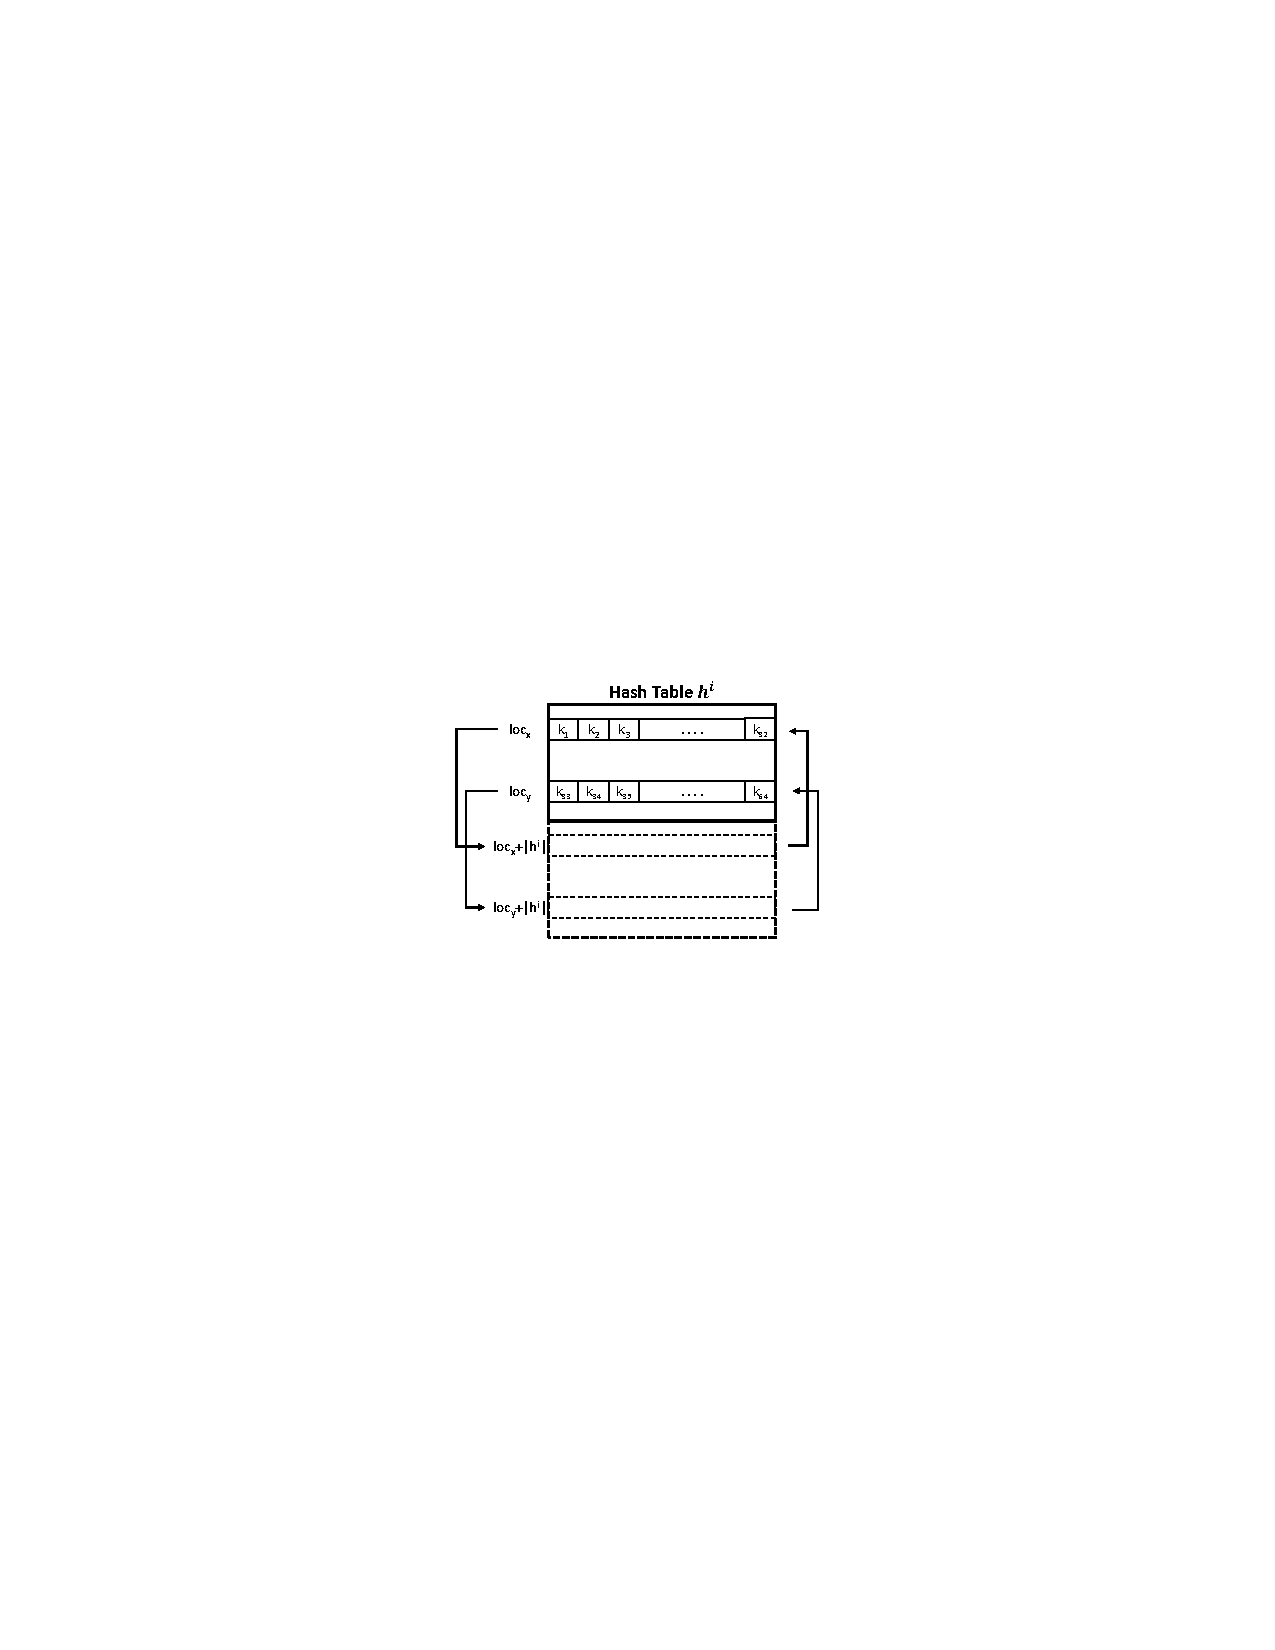
\includegraphics[width=0.3\textwidth]{fig/Upsize.pdf}
	\caption{Illustration for upsizing and downsizing.}
	\label{fig:upsize}
\end{figure}
\vspace{1mm}\noindent\textbf{Upsizing.} 
We introduce a conflict-free rehashing strategy for the upsizing scenario. 
Figure~\ref{fig:upsize} presents an illustration for upsizing a hash table $h^i$. 
As we always double the size for $h^i$, 
a KV pair which originally resides in bucket $loc$ could be rehashed to bucket $loc+|h^i|$ or stay in the original bucket. 
With this observation, we assign a warp for rehashing all KV pairs in bucket to fully utilize the cache line size. 
Each thread in the warp corporately takes a KV pair in the bucket and relocates the KV pair if necessary.
Moreover, the rehashing does not trigger any conflict since KV pairs from two distinct buckets before upsizing cannot be rehashed to the same bucket.  
Thus, the locking of a bucket is not required and we can make use of the full device memory bandwidth for the upsizing process.  

Note that after upsizing hash table $h^i$, its filled factor $\theta_i$ is cut to half, which could break the balancing condition emphasized in Theorem~\ref{them:balance}. Nevertheless, we use the sampling strategy for subsequent KV insertions, where each insertion is allocated to table $i$ with a probability proportional to $n_i/\binom{m_i}{2}$, to recover the balancing condition. In particular, $m_i$ remains the same while $n_i$ doubles after upsizing, the scenario leads to double the probability of inserting subsequent KV pairs to $h^i$. 


\vspace{1mm}\noindent\textbf{Downsizing.}
Downsizing the hash table $h^i$ is a reverse process of upsizing $h^i$. We note that there is always room to relocate KV pairs in the same table for upsizing. 
In contrast, downsizing may rehash some KV pairs to other hash tables, especially when $\theta_i > 50\%$.
Since the KV pairs located in $loc$ and $loc+|h^i|$ are hashed to $loc$ in the new table, there could be cases the KV pairs exceeds the size of a single bucket. 
Hence, we first assign a warp to accommodate KV pairs that can fit the size of a single bucket. Similar as upsizing, it does require locking since there will be no thread conflict on any bucket. 
For the remaining KV pairs which cannot fit in the downsized table, called \emph{residuals}, we insert them into other subtables.
To make sure no conflict occurs between inserting residuals and processing the downsizing subtable, which are both executed in a single kernel, we exclude the downsizing subtable when inserting the residuals. 
Take an example when we have three subtables and one of them is being downsized. 
We only insert the residuals to the remaining two subtables. 


%To safeguard the balancing condition, we devise a different rehashing strategy for downsizing. 
%For all KV pairs in bucket $loc \geq |h^i|/2$ for table $i$ to be downsized, we assign a thread to rehash and reinsert a KV pair using Algorithm~\ref{algo:insert}. 
%In this way, we achieve the balancing condition at the expense of locking a bucket when reinserting a KV pair. 

\vspace{1mm}\noindent\textbf{Complexity Analysis.}
Given a total of $m$ elements in the hash tables, upsizing/downsizing rehashes at most $m/d$ KV pairs. 
For inserting/deleting these $m$ elements, the number of rehashes is bounded by $2m$. 
Thus, the amortized complexity for inserting $m$ elements is still $O(1)$.
